\newpage
\appendix
\appendixpage
\addappheadtotoc

\chapter{Project management forms}
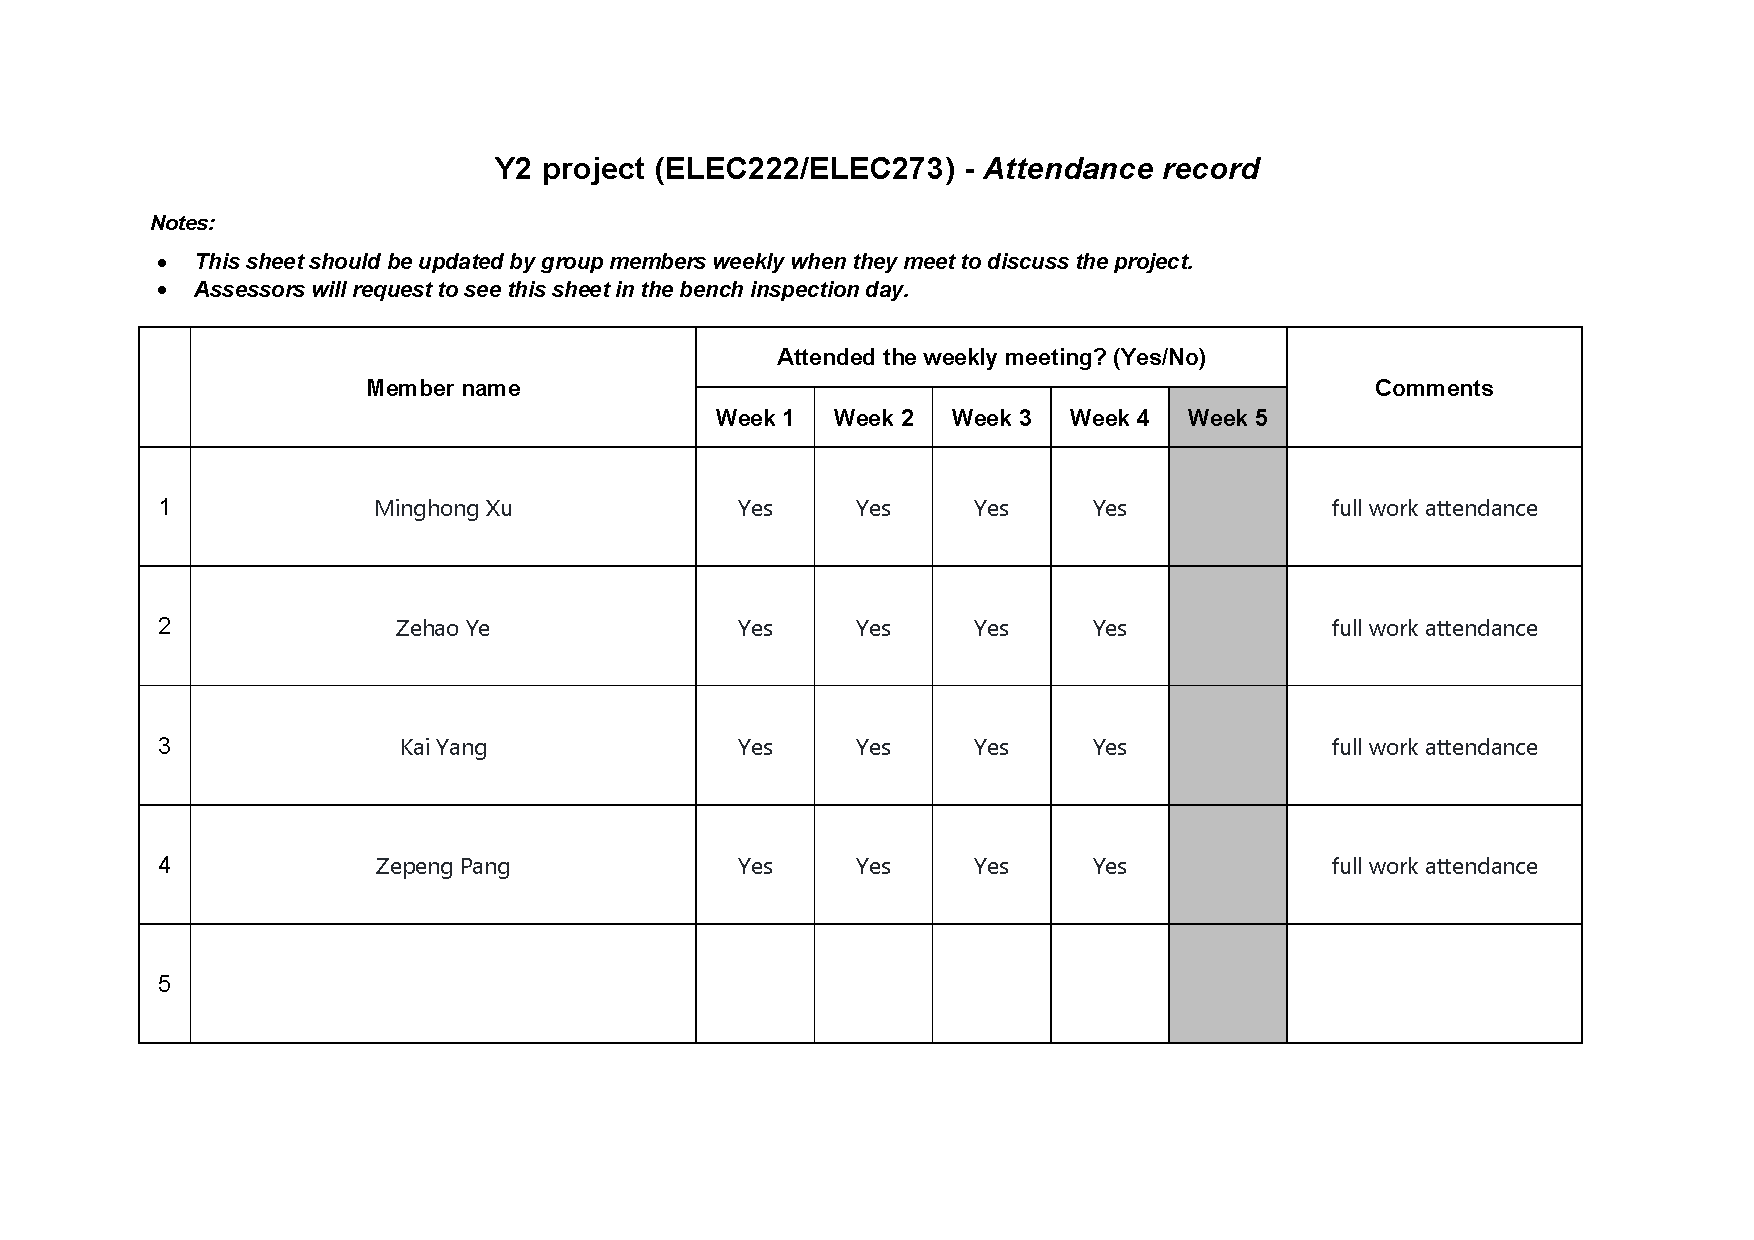
\includepdf[pages=-]{../proj_mgmt_forms/attendance_record.pdf}
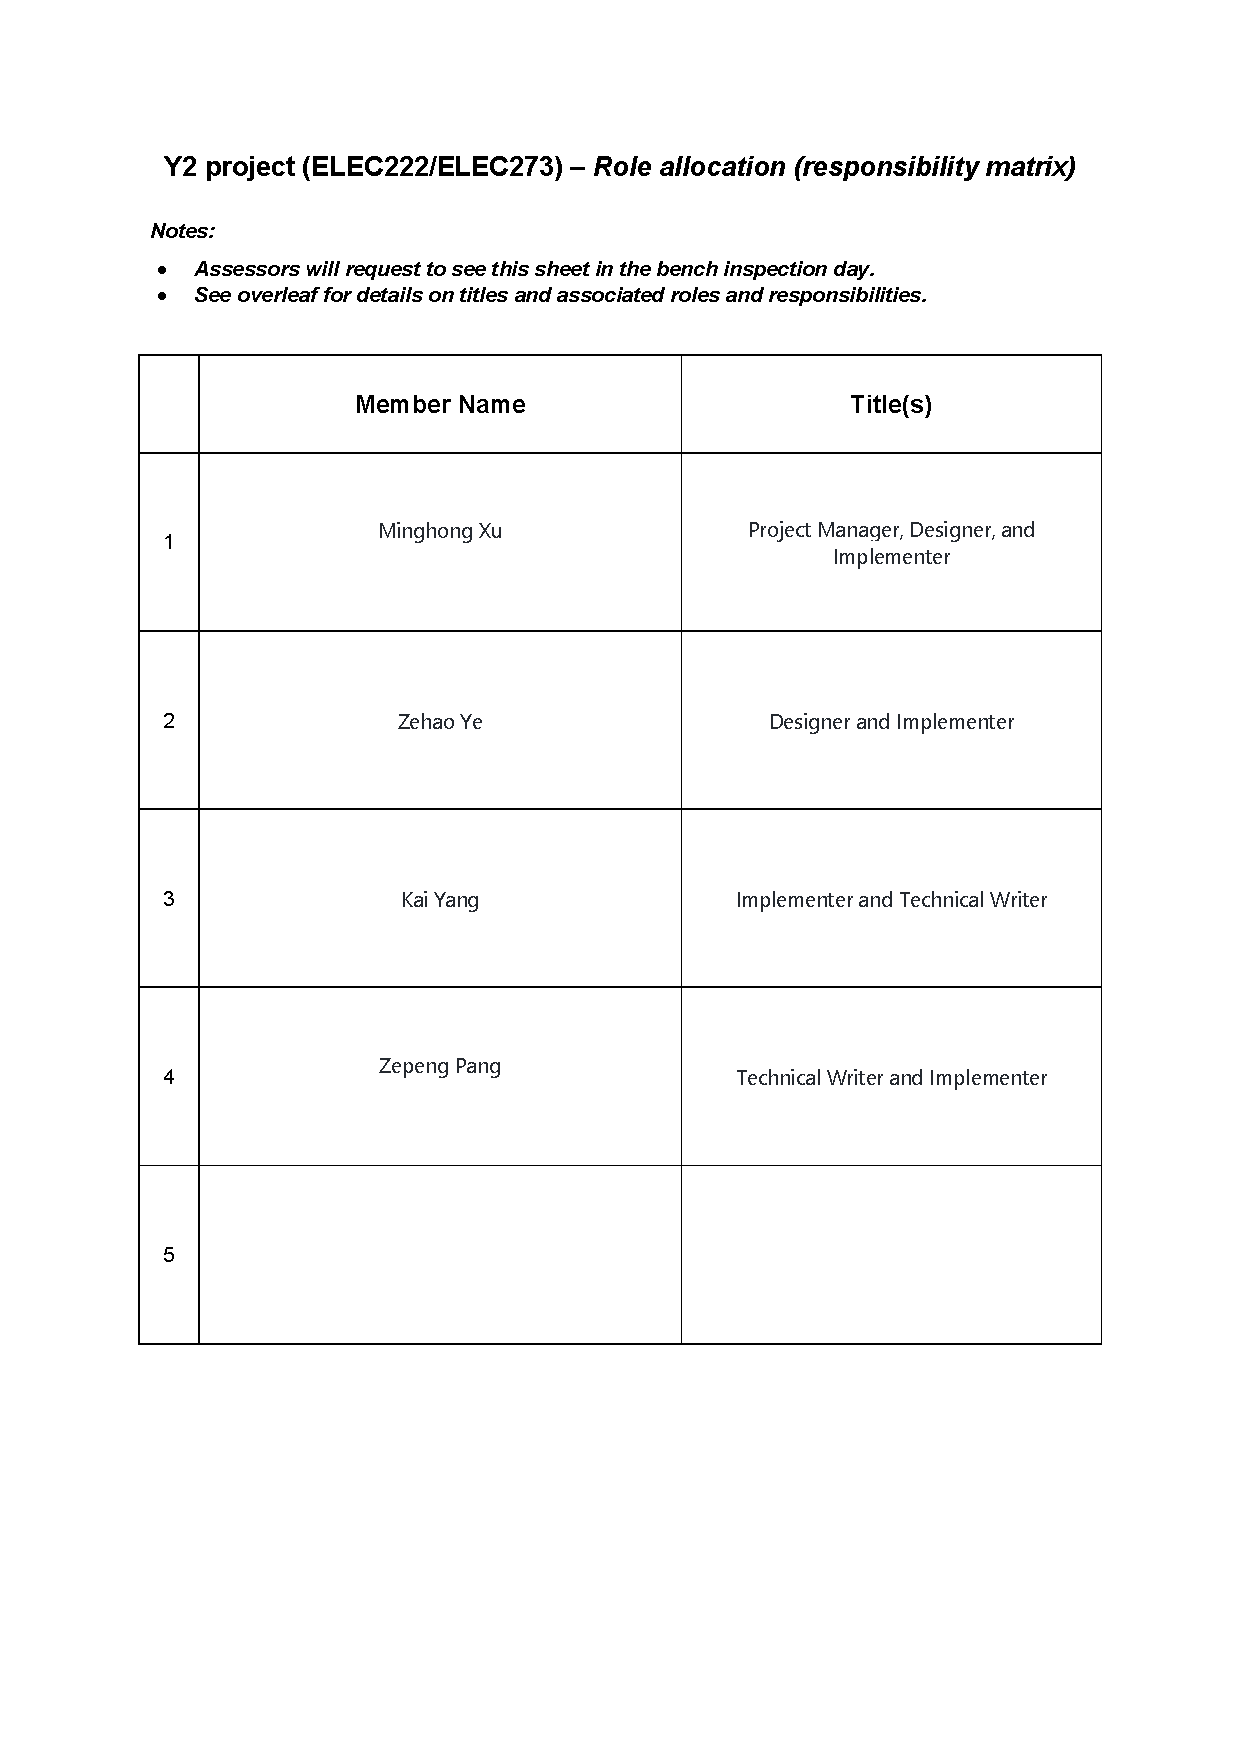
\includepdf[pages=-]{../proj_mgmt_forms/role_allocation.pdf}
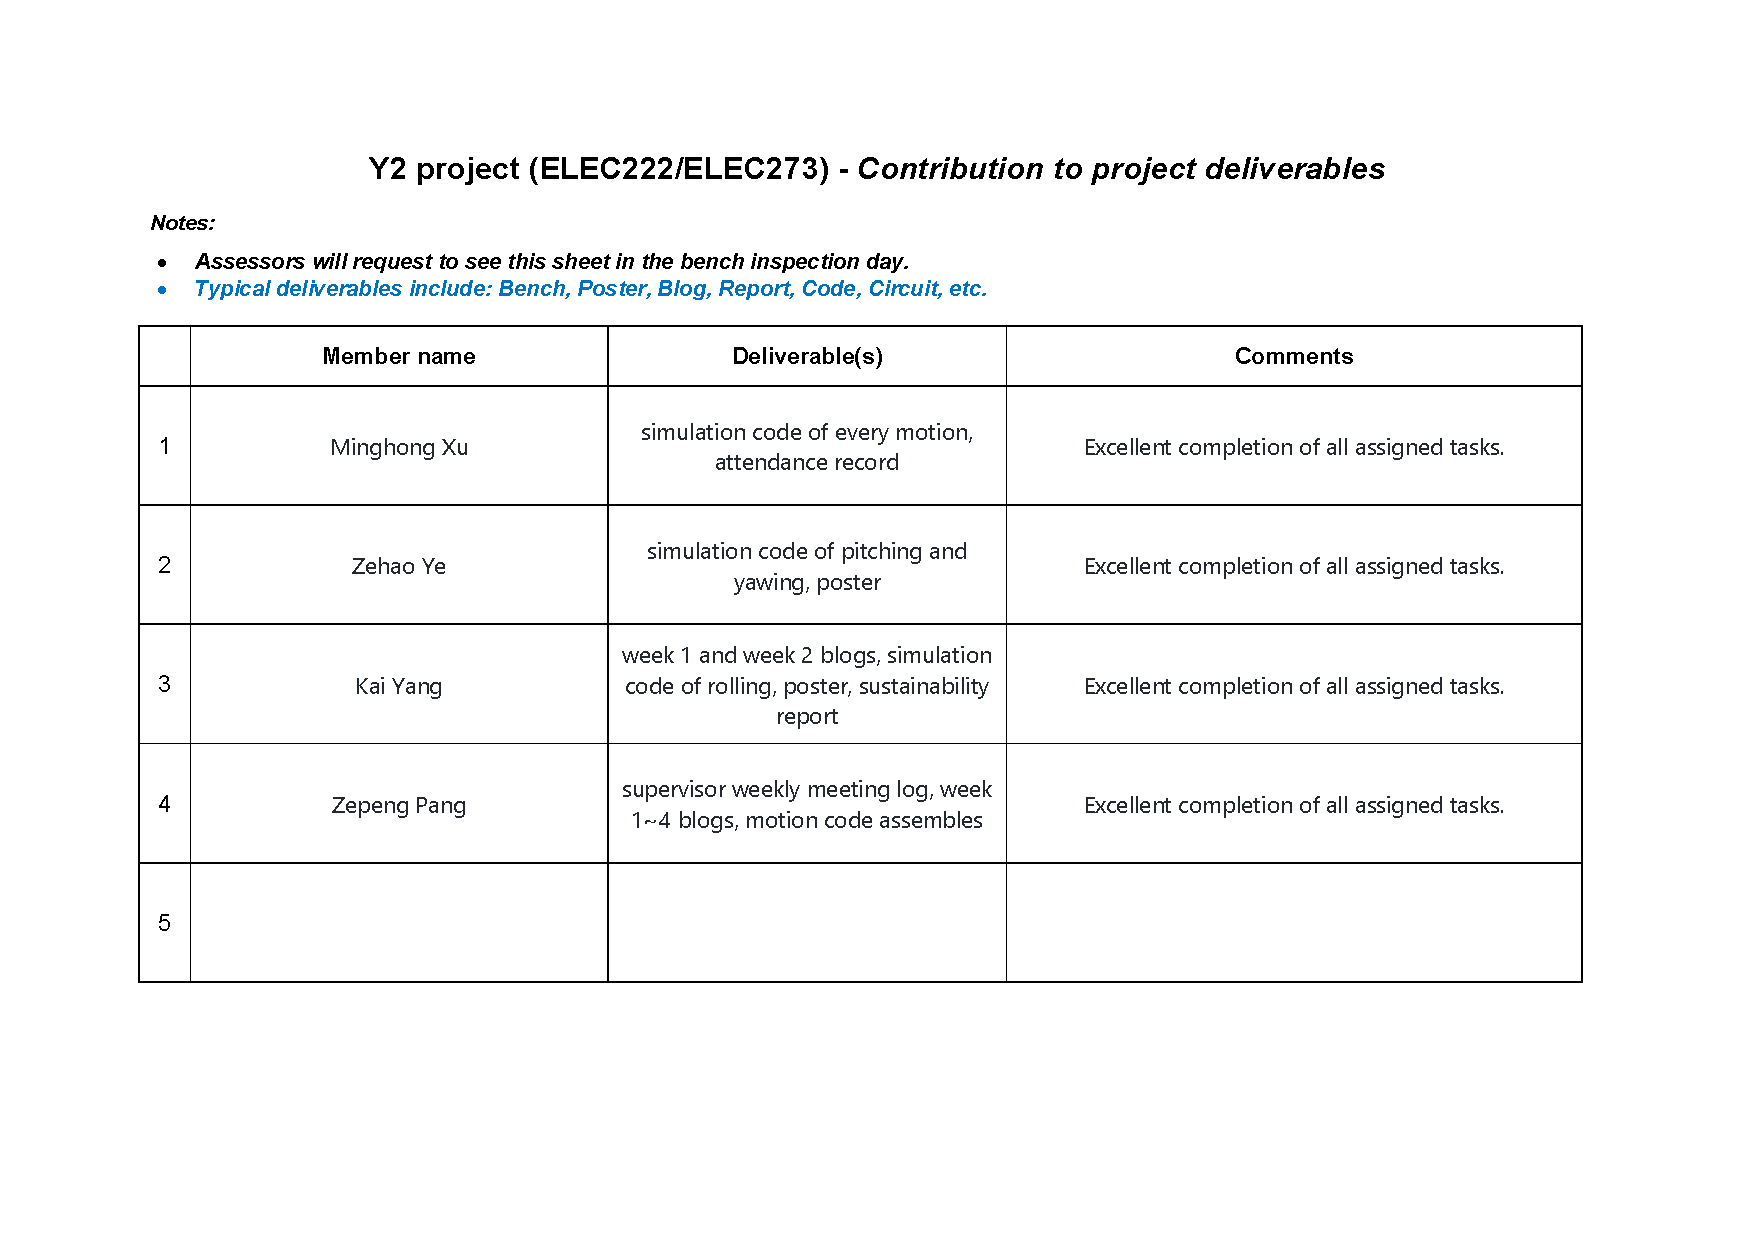
\includepdf[pages=-]{../proj_mgmt_forms/contribution_to_project_deliverables.pdf}
\includepdf[pages={2}]{../proj_mgmt_forms/advisor_meeting_log_weeks_1_2.pdf}
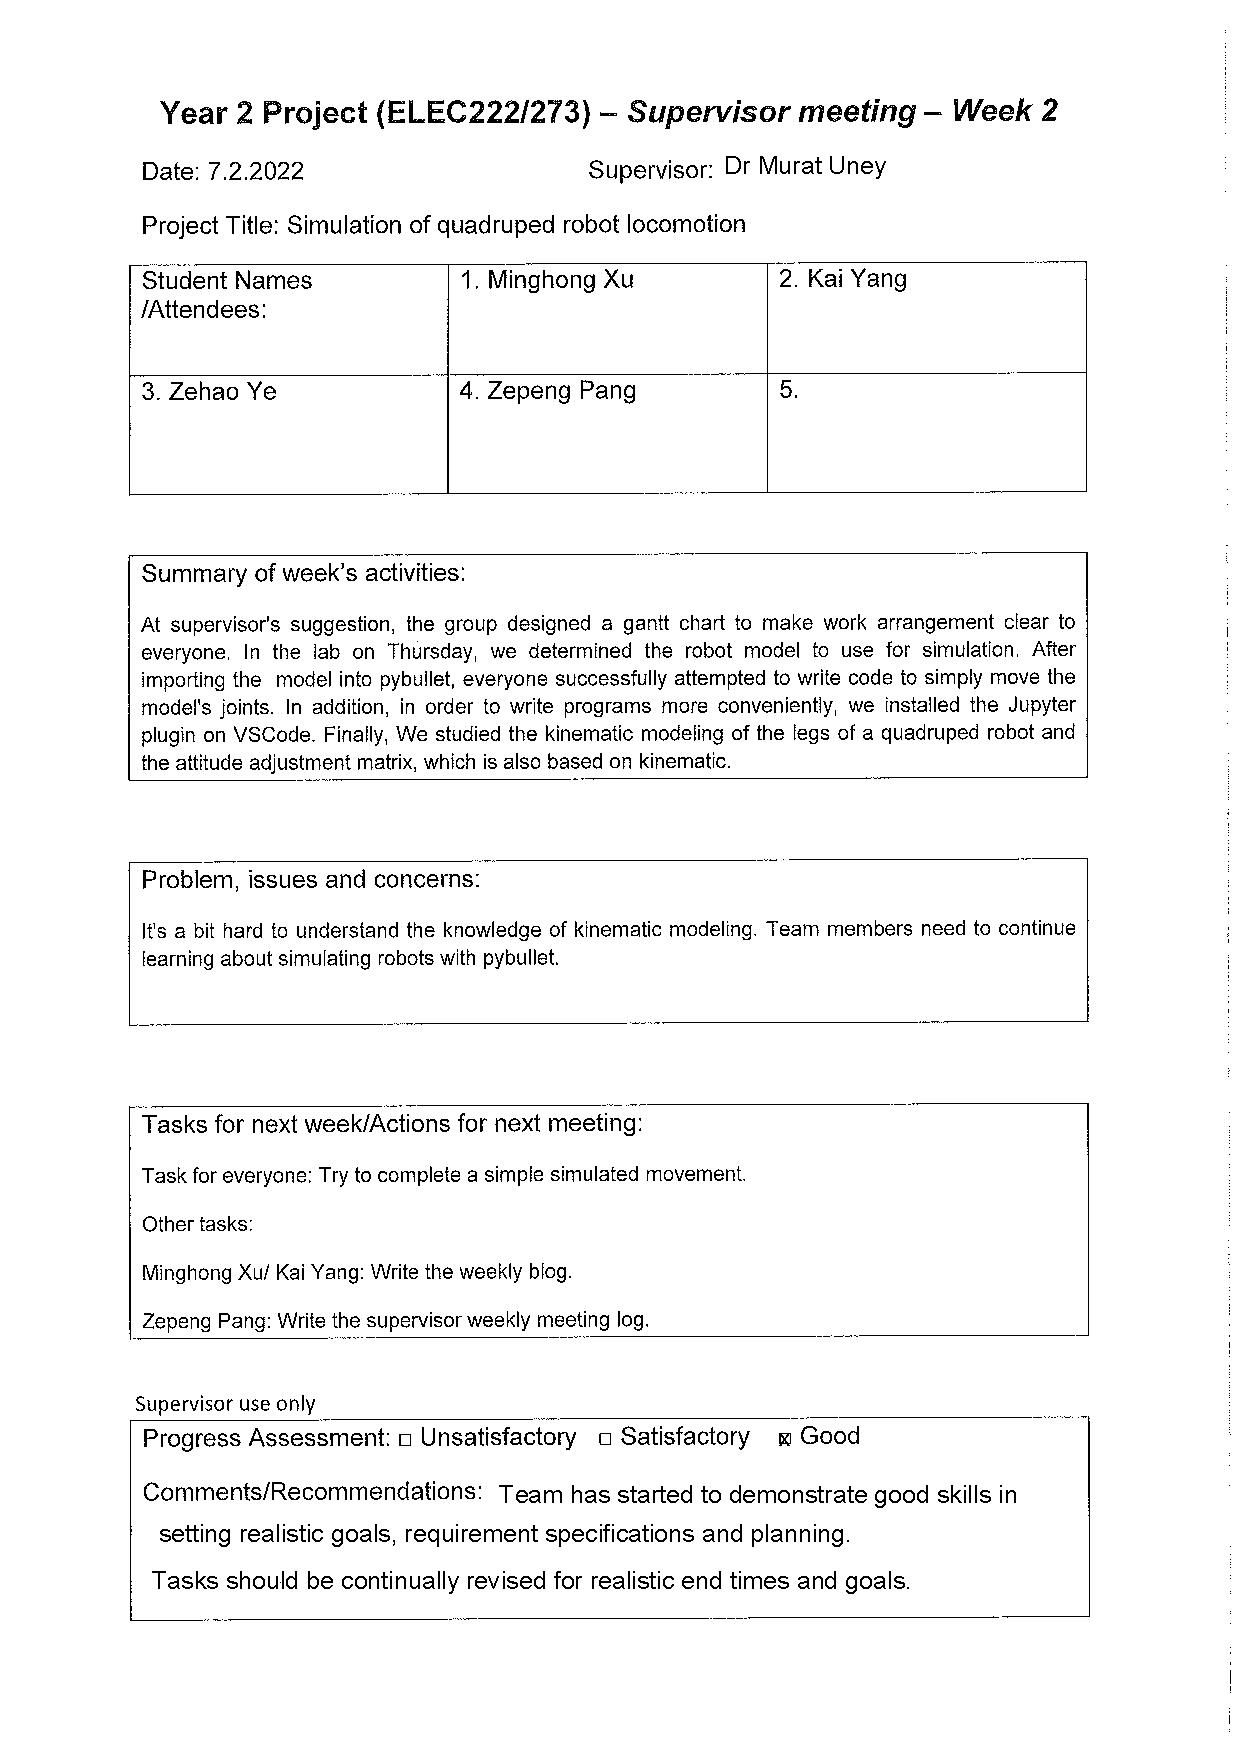
\includepdf[pages={1}]{../proj_mgmt_forms/advisor_meeting_log_weeks_1_2.pdf}
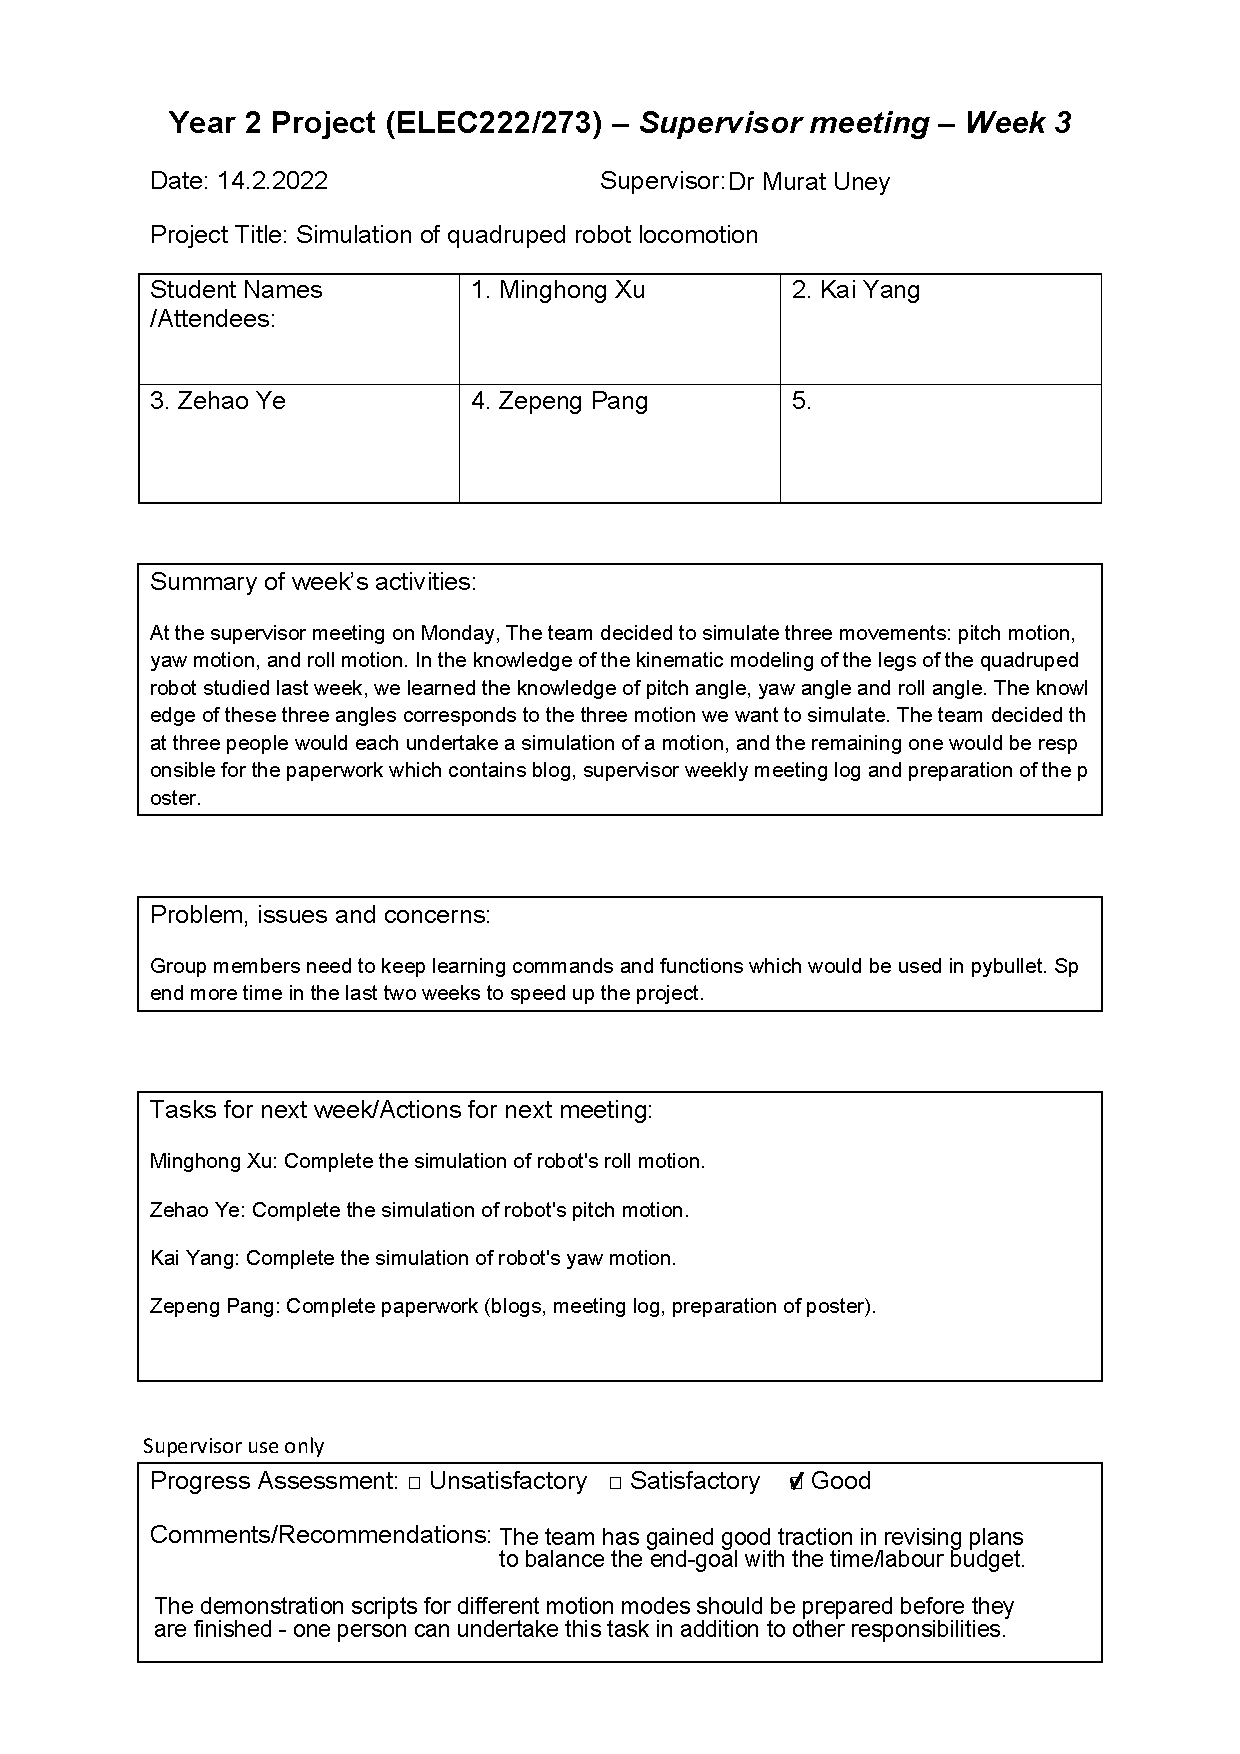
\includepdf[pages=-]{../proj_mgmt_forms/advisor_meeting_log_week_3.pdf}
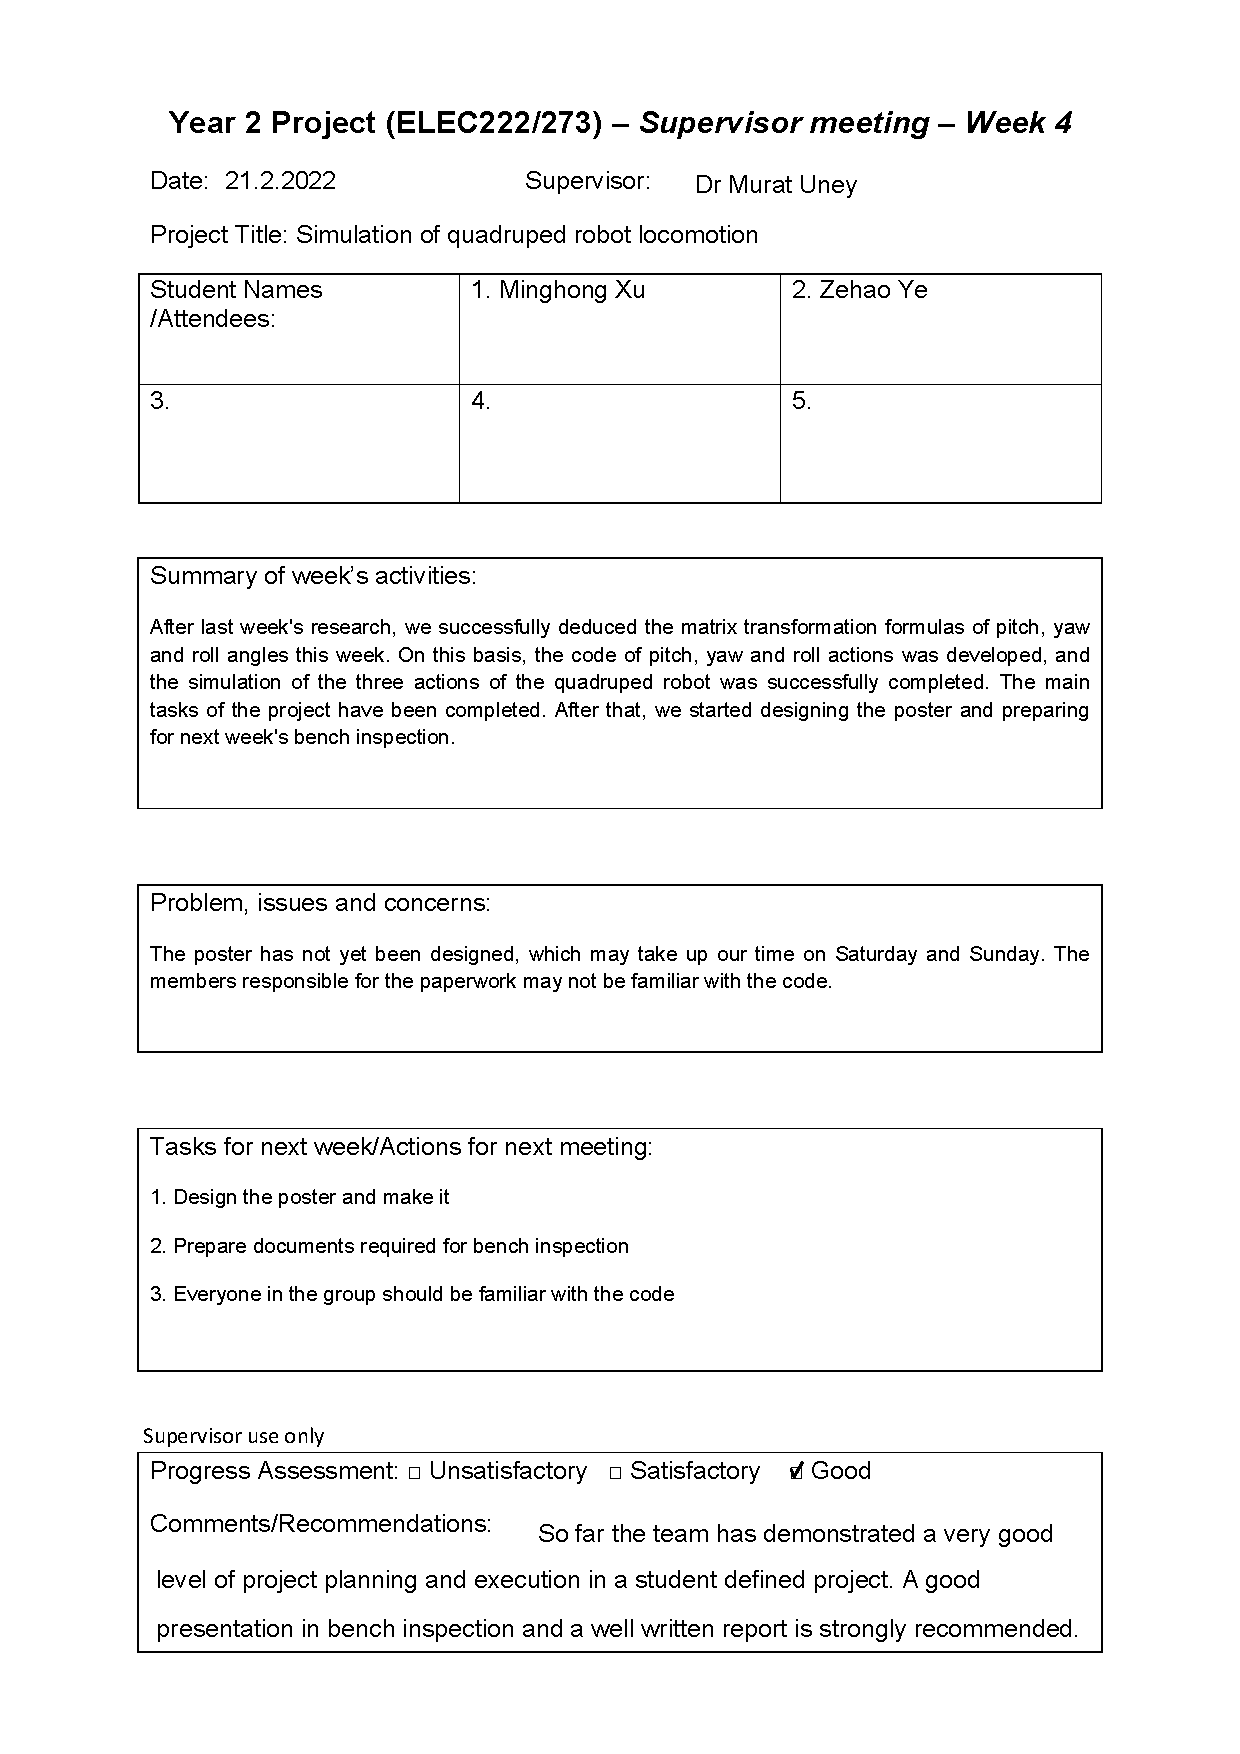
\includepdf[pages=-]{../proj_mgmt_forms/advisor_meeting_log_week_4.pdf}

\chapter{Individual contributions to the project}
\section{Minghong Xu}
\section{Zehao Ye}
In this group project, I am mainly responsible for three aspects, which are quadrupedal locomotion simulation, presentation and report. From the perspective of quadrupedal locomotion simulation, I have completed the forward and inverse kinematics derivation and matrix derivation of some parts of pitch, yaw and roll actions. The part I participated in most was pitching. Meanwhile, debug parameter section was mainly designed by me. From the perspective of presentation, I drew the poster through software. In the poster, except that the pictures of the modelling part were made by Yang Kai, other parts were completed by me. From the perspective of report, I wrote the results and analysis section. In addition, the limitations of the discussion and conclusion section are also completed by me.

\section{Zepeng Pang}
\section{Kai Yang}
